\documentclass[review]{elsarticle}
\biboptions{authoryear}

\usepackage{amsmath,amssymb}
\usepackage{graphicx}
\usepackage{booktabs}
\usepackage{multirow}
\usepackage{placeins}
\usepackage{lineno}
\modulolinenumbers[5]

\journal{Electronic Commerce Research and Applications}

\bibliographystyle{elsarticle-harv}

\begin{document}

\begin{frontmatter}

\title{When AI Shops with AI: Buyer-Seller Agent Negotiation and Market Outcomes in Agentic Commerce}

% Author name, affiliation, and acknowledgments are withheld from this
% copy for double-anonymized review, per the ECRA Guide for Authors.
% See the separate title page file (titlepage.tex) submitted alongside
% this manuscript.

\begin{abstract}
A growing share of online purchases will soon be negotiated not between a person and a merchant, but between a buyer's shopping agent and a seller's pricing agent. This paper asks what happens to prices, welfare, and market structure when that shift occurs, using a matched agent-based computational economics (ACE) simulation of 105,600 transactions across 80 replicate markets, each run through five institutional regimes that span the space between today's posted-price web store and a fully autonomous, multi-seller negotiation. Moving from limited human-style search to full AI-mediated search raises total welfare by improving buyer-seller matching, but pure price bargaining on top of that search is almost perfectly redistributive: it reallocates surplus between buyer and seller without enlarging the pie. Allowing agents to negotiate over bundles and delivery terms in addition to price, however, does enlarge it, by roughly 13.6 welfare units per transaction, a genuine efficiency gain from a richer negotiation space rather than a transfer. That efficiency gain has a darker mirror: as sellers' agents learn more about a given buyer, the buyer's share of the surplus falls from 84 percent to 68 percent, a direct and statistically precise price-discrimination effect. Full-market AI search also concentrates trade sharply among a small number of winning sellers (a win-share Herfindahl index rising from about 0.10 to 0.60), though allowing sellers to compete for the buyer's attention simultaneously partially reverses this concentration. Two further findings speak directly to policy-relevant fears about agentic commerce: buyers who share a common buyer-side agent provider capture a modestly larger surplus share than independent buyers, a real monopsony effect; and while shared seller-agent infrastructure does not mechanically compress market-wide price dispersion, it does explain roughly 45 percent of the markup variance among sellers on that infrastructure, evidence of real correlation without evidence of collusion. A smaller, exploratory pilot in which real Gemini and OpenRouter language models negotiate directly, rather than following the paper's rule-based protocol, corroborates the central bundling result: conditional on reaching a deal, multi-attribute negotiation again outperforms price-only bargaining. Together, the results suggest that the economic consequences of agentic commerce depend less on whether AI agents are present than on which specific institutional rules govern how they search, bargain, and disclose information.
\end{abstract}

\begin{keyword}
agentic commerce \sep AI shopping agents \sep multi-agent negotiation \sep agent-based computational economics \sep algorithmic pricing \sep market design
\end{keyword}

\end{frontmatter}

\section*{Highlights}
% Elsevier submission systems require Highlights as a separate uploaded
% file (3-5 bullets, max 85 characters each); included here for
% completeness of the manuscript copy.
\begin{itemize}
\item AI-mediated search raises welfare; pure price bargaining only redistributes it
\item Multi-attribute negotiation creates surplus: +13.6 welfare units versus price-only
\item Seller information advantage cuts buyer surplus share from 84\% to 68\%
\item Full-market search raises seller concentration sixfold; competition offsets it
\item Shared buyer- and seller-agent infrastructure shifts bargaining power, not collusion
\end{itemize}

\linenumbers

\section{Introduction}

Imagine a buyer who wants a new television. Twenty years ago she would have visited two or three stores, compared a handful of models, and either paid the sticker price or haggled a little at the register. Today she opens a handful of browser tabs and a comparison site does the work of visiting every store at once. Tomorrow, on the trajectory that most large e-commerce and AI platforms are currently building toward, she will simply tell a shopping agent her budget and preferences and let it search, negotiate, and transact on her behalf. On the other side of that transaction, an increasing number of merchants already price and reprice using algorithmic pricing engines, and a growing number are experimenting with agents that can negotiate directly with a buyer's agent rather than simply posting a take-it-or-leave-it price. Both trends are old; what is new is the prospect that they meet in the same transaction, with an AI agent representing the buyer negotiating against an AI agent representing the seller, and no human present at the point of sale at all.

This paper asks a simple question with a genuinely open answer: does it matter, for prices, welfare, and market structure, precisely how that meeting is organized? The intuition that "AI agents will change e-commerce" is by now close to a truism, echoed across the trade press and the emerging academic literature on agentic markets \citep{bichler2026agentic,shahidi2025coasean,hadfield2025economy}. It is a much less obvious claim that the institutional details of the meeting -- how much of the market a buyer's agent actually searches, whether the resulting price is posted or bargained, whether the bargaining space includes only price or also bundles and delivery terms, and whether the buyer's or seller's agent is one of many independent implementations or one of a handful of shared platforms serving many principals at once -- determine whether that change helps buyers, helps sellers, or mostly just reshuffles who captures a roughly fixed amount of surplus. Untangling those institutional details from the mere presence of AI is the central contribution of this paper.

The question has an obvious empirical difficulty: agentic commerce, in the sense of autonomous buyer and seller agents transacting without a human in the loop, is not yet common enough to observe at scale, and the platforms that are beginning to deploy something like it treat their negotiation logic as a trade secret. Two research strategies are available in the interim. One is to build small experimental testbeds and have real large language models negotiate inside them, which has the appeal of studying the actual technology but the limitation that current testbeds are necessarily small, and the artifacts of any one model's training and prompting can be mistaken for a general economic finding \citep{bianchi2024negotiationarena,zhu2025automated,bansal2025magentic}. The other is to build an explicit, parametrized model of the market mechanism itself -- an agent-based computational economics (ACE) approach in the tradition surveyed by \citet{tesfatsion2006agent} -- and ask what that mechanism implies for prices and welfare under full experimental control. This paper takes the second route as its primary empirical strategy, and supplements it with a small, explicitly exploratory pilot of the first kind, run over the same underlying environment, as a check on whether the mechanism-level story survives contact with an actual, non-scripted negotiator.

The simulation crosses five institutional regimes -- posted price with limited search, AI-assisted full-market search with no bargaining, bilateral price-only bargaining, bilateral multi-attribute bargaining, and competitive multi-seller solicitation -- with seller information about the buyer, whether the negotiation space includes non-price attributes, and whether either side of the market is served by a small number of shared agent providers or a large number of independent ones. Every replicate market is run through every applicable combination of these conditions with the same drawn population of buyers and sellers, so that differences across regimes reflect the institutional rule change itself rather than a different draw of who happened to be trading with whom. The result is 105,600 simulated transactions across 80 replicate markets, generating the six empirical findings summarized in the abstract: search improves matching efficiency; price-only bargaining is close to purely redistributive; multi-attribute bargaining genuinely creates surplus; richer seller information about the buyer extracts surplus from her; full AI-mediated search concentrates trade among fewer winning sellers, an effect that competitive multi-seller solicitation partially undoes; and buyer-side and seller-side agent-provider concentration both leave detectable, but importantly different, fingerprints on the resulting prices.

The paper's contribution is therefore not to claim that AI agents will make markets more efficient or less fair in general, a claim the results below suggest is not well posed, but to show which specific design choices move each of those two outcomes, and by how much, inside one consistent and fully reproducible environment. Section 2 situates the paper against four adjacent literatures: e-commerce search and recommendation, the nascent literature on agentic markets, algorithmic pricing and collusion, and the older literatures on price discrimination and bilateral negotiation that this new setting recombines. Section 3 develops the formal model, the five institutional regimes, and seven hypotheses that map directly onto the empirical tests that follow. Section 4 describes the simulation and the supplementary LLM-agent pilot, and is deliberately explicit about the difference in what each can and cannot claim to show. Section~\ref{sec:results} reports the results, including a set of robustness checks added to test the paper's own structural assumptions directly; Section~\ref{sec:discussion} discusses their implications for platform design and competition policy; Section~\ref{sec:limitations} states the paper's limitations; and Section~\ref{sec:conclusion} concludes with the empirical work that would be needed to move from a mechanism-level claim to a claim about any specific deployed system.

\section{Literature Review}

\subsection{Search costs and matching in electronic markets}

The starting premise of this paper -- that reducing the cost of search should, in itself, be welfare-improving -- rests on a literature that predates AI shopping agents by decades. \citet{stigler1961economics} first formalized the idea that costly search generates equilibrium price dispersion even among sellers of an identical good, because no buyer can profitably examine every seller. \citet{bakos1997reducing} showed that electronic marketplaces, by collapsing the marginal cost of examining one more seller toward zero, should compress that dispersion and shift surplus toward buyers, a prediction that generated a lively empirical debate about whether real online markets actually behaved that way; \citet{harrington2001comment}'s comment on Bakos's model is a useful reminder that the mapping from "search is cheaper" to "buyers do better" depends on exactly how search frictions are modeled, a caution this paper takes seriously by treating search breadth as one dial among several rather than the only one that matters. More recent work on AI-mediated recommendation and choice, such as \citet{kim2023decisions}'s study of choice overload in conversational recommendation, extends the search-cost logic into the current generation of AI-assisted shopping tools, and is one of the few empirical anchors available for how an AI intermediary changes buyer decision quality rather than just buyer effort.

This paper's regimes M0 and M1 are a direct, if stylized, operationalization of that debate: M0 restricts the buyer's agent to examining a small, fixed number of sellers, mimicking a human shopper's practical search limit, while M1 gives the buyer's agent costless access to the entire market. The resulting welfare gain from M0 to M1, and the accompanying fall in the average transaction price, replicate the classic search-cost story quantitatively rather than just qualitatively, and set up the paper's more novel question: once search is essentially free, as it plausibly becomes once an AI agent is doing it, does adding bargaining on top of that search create any further gains, or does it only redistribute the ones search already delivered?

\subsection{Agentic commerce and markets with AI agents}
\label{sec:litreview-agentic}

A body of work published almost entirely within the last two years has begun to ask what happens when the buyer, the seller, or both are themselves autonomous software agents rather than a human using a tool. \citet{bichler2026agentic} frames the central open question of this literature precisely: that agentic markets could in principle deliver large efficiency gains from better search and faster negotiation, but that "gains are not automatic" and depend on the market's institutional design, a framing this paper takes as its organizing hypothesis and its title's implicit claim. \citet{shahidi2025coasean} develop a formal argument, which they term the Coasean Singularity, that falling transaction costs from AI intermediation should push real markets toward the frictionless, transfer-neutral benchmark that Coase's theorem describes in the limit -- a benchmark against which this paper's finding that price-only bargaining is nearly perfectly redistributive is a striking, if partial, confirmation. \citet{hadfield2025economy} take a broader view of an emerging "economy of AI agents" and the institutional infrastructure, from identity and liability to contracting norms, that such an economy will require. Closer to this paper's specific empirical object, \citet{allouah2026aiagent} directly study what a shopping AI agent actually buys and how its choices are biased relative to a human's, an important complement to a paper like this one that instead holds buyer preferences fixed and varies the market's rules. \citet{bansal2025magentic} and \citet{zhu2025automated} each build open experimental testbeds -- Magentic Marketplace and an agent-to-agent consumer negotiation benchmark, respectively -- for studying real deployed language models transacting with each other, the same broad research strategy this paper's supplementary LLM pilot adopts at a far smaller scale. \citet{bichler2025agenticgame} model the game-theoretic dynamics of learning agents in agentic markets directly, a formally richer complement to this paper's rule-based approach. \citet{bianchi2024negotiationarena} is an earlier and by now foundational benchmark for evaluating how well large language models negotiate against each other or against scripted opponents, and its finding that negotiation outcomes are highly sensitive to which specific model is playing which role is directly relevant to this paper's own small-scale finding, in Section~\ref{sec:results-llm}, that a Gemini-versus-Gemini pairing, an OpenRouter-versus-OpenRouter pairing, and a mixed pairing do not behave identically. Finally, \citet{bostoen2026futureproof} examine how well existing digital-market regulation, specifically the European Union's Digital Markets Act, anticipates a world of autonomous negotiating agents, a question this paper's concentration findings speak to directly in Section~\ref{sec:discussion}.

A "buyer-agent provider" or "seller-agent provider" serving many principals at once, in the sense this paper's concentration treatments operationalize, is structurally an intermediary platform, and the two-sided-markets literature founded by \citet{armstrong2006competition} is the natural theoretical home for that observation: platforms serving multiple sides of a market internalize cross-side effects in ways that a population of fully independent agents does not, which is precisely the mechanism this paper's buyer- and seller-concentration results (Section~\ref{sec:results-buyerconc}, Section~\ref{sec:results-sellerconc}) are designed to probe empirically, even though the paper does not build a full platform-pricing model of its own.

What is missing from this fast-moving literature, and what this paper tries to supply, is a controlled comparison across institutional regimes using a single population of buyers and sellers held fixed across treatments. Papers that build testbeds for real language models are, almost by construction, exploring one or a few configurations of that testbed rather than sweeping systematically across the space of market designs; this paper inverts that trade-off, sacrificing the realism of an actual deployed language model as the primary evidence in exchange for full experimental control over exactly which institutional lever is being turned.

\subsection{Algorithmic pricing and the collusion question}
\label{sec:litreview-collusion}

A parallel and more mature literature asks whether algorithmic pricing agents, even without any agentic buyer on the other side, can produce collusive-like outcomes without any explicit agreement, human intent, or even communication among the pricing algorithms. \citet{calvano2020artificial} showed in a landmark reinforcement-learning simulation that independently trained pricing algorithms could learn to sustain supra-competitive prices through reward-punishment schemes that require no explicit signaling, a result extended to settings with imperfect monitoring in \citet{calvano2021algorithmic}. \citet{klein2021autonomous} demonstrated a similar tacit-collusion result for Q-learning agents under sequential pricing, and \citet{brown2023competition} brought some of this theoretical concern to real-world grounding with evidence on how actual algorithmic pricing software affects retail gasoline competition. \citet{sanchezcartas2025ai} extend this line of inquiry to platform competition specifically, which is closer to this paper's e-commerce setting.

This paper's own concentration findings sit adjacent to, but are conceptually distinct from, that collusion literature. The algorithmic-collusion papers ask whether independent pricing agents can converge to a joint-profit-maximizing outcome without communicating; this paper instead asks what happens when sellers are not fully independent to begin with, because a subset of them share a common third-party agent provider, and finds a genuinely nuanced answer, developed fully in Section~\ref{sec:results-sellerconc}, in which shared infrastructure correlates within-network markups without mechanically compressing overall market-wide price dispersion. \citet{harrington2026hubandspoke} shows formally that hub-and-spoke collusion can arise when sellers share a third-party pricing algorithm even without the sellers themselves communicating -- a mechanism structurally closer to this paper's shared-provider setup than to the independently-learning agents studied by \citet{calvano2020artificial}, and one this paper returns to directly in Section~\ref{sec:discussion}, which argues that conflating correlation with collusion outright would overstate what the simulation shows, without treating the two as unrelated either.

\subsection{Personalization and price discrimination}
\label{sec:litreview-personalization}

The seller-information dimension of this paper's design draws on an established literature on how much a firm can extract from a buyer once it can infer that buyer's willingness to pay. \citet{bergemann2015limits} characterize the full range of consumer-surplus and producer-surplus outcomes that price discrimination can theoretically produce as a function of how much the seller knows about buyer valuations, a range this paper's own information-level treatment -- from a seller who knows nothing beyond its own cost to one that observes the buyer's urgency and purchase history -- is designed to traverse empirically rather than just characterize theoretically. \citet{dube2023personalized} bring this question to real personalized-pricing data and find that welfare effects of personalization depend heavily on the specific pricing technology in use, a caution against assuming personalization is uniformly good or bad for consumers. \citet{acquisti2005conditioning} study the specific mechanism of conditioning price on purchase history, directly analogous to this paper's "history-aware" seller information level, and find, as this paper does, that loyalty signals can be turned against the buyer rather than rewarded. \citet{akerlof1970market}'s classic analysis of information asymmetry, though framed around quality rather than willingness to pay, is the conceptual ancestor of this entire literature: whichever side of a transaction knows more has a structural advantage, and an AI agent's central economic function is to change who knows what.

\subsection{Negotiation theory and transaction costs}
\label{sec:litreview-negotiation}

Finally, the paper's bilateral bargaining regimes rest on a negotiation-theoretic foundation reaching back to \citet{nash1950bargaining}'s axiomatic characterization of the bargaining outcome and \citet{rubinstein1982perfect}'s non-cooperative alternating-offers model, which showed that patience and the cost of delay, not raw bargaining power alone, determine how a fixed surplus gets split between two parties. \citet{myerson1983efficient}'s impossibility result -- that no mechanism can guarantee both individual rationality and full efficiency in bilateral trade under two-sided private information -- is the deeper theoretical reason a real bargaining protocol can leave value on the table at all, and is the backdrop against which this paper's price-only bargaining regime (M2) should be read: it is not that price-only bargaining is inefficient by some avoidable design flaw, but that expanding the space of what can be traded, as in the multi-attribute regime (M3), is one of the few generally available ways around a private-information bargaining problem that Myerson-Satterthwaite shows cannot otherwise be solved away. The economics of exactly why expanding the bargaining space this way creates value has its own dedicated literature: \citet{adams1976commodity} first showed that bundling goods together can raise a seller's profit by smoothing out heterogeneity in buyer valuations, and \citet{bakos2000bundling} extended this logic specifically to internet commerce, showing that bundling can generate real efficiency gains, not just extractive ones, when the goods bundled have low marginal cost relative to their value -- precisely the condition this paper's own sensitivity analysis (Section~\ref{sec:robustness}) shows determines whether the multi-attribute mechanism here raises or lowers total welfare. The simulation's actual negotiation protocol is a parametrized, monotonic-concession model in the tradition of \citet{faratin1998negotiation}, whose negotiation decision functions remain the standard reference for modeling how an autonomous agent should concede over time as a function of its own urgency and its beliefs about its counterpart. \citet{williamson1981economics} and \citet{coase1937nature} complete the theoretical picture from the institutional-economics side: both argue that the boundaries of firms and the design of contracts exist to economize on the transaction costs of negotiating, monitoring, and enforcing exchange, which is precisely the cost category that an AI negotiating agent is built to reduce. Taken together, this literature anticipates, rather than is merely restated by, this paper's central empirical pattern: because a bilateral bargain over a fixed pie is, in Rubinstein's framework, a transfer problem, a bargaining regime layered on top of an already-efficient search regime should not be expected to raise total welfare on its own, and the simulation's M1-versus-M2 comparison (Section~\ref{sec:results-search}) is best read as confirming that this classical prediction survives being embedded in a full market-matching environment, not as an independent discovery. Any welfare gain from negotiation, if the theory is right, has to come from expanding what is actually being bargained over, which is exactly the test that distinguishes this paper's price-only regime (M2) from its multi-attribute regime (M3) -- and, as Section~\ref{sec:robustness} shows, that gain is itself conditional on the bundled good being reasonably cheap to provide relative to its value, not guaranteed by the mere act of expanding the bargaining space.

\section{Model and Hypotheses}

\subsection{Buyers, sellers, and utility}
\label{sec:model-utility}

Each simulated buyer $i$ has a private valuation $v_i$ for one unit of a homogeneous product, drawn independently across buyers, and a budget ceiling slightly above that valuation. Each seller $j$ has a private unit cost $c_j$ and a minimum acceptable markup over that cost, both drawn independently across sellers. When a transaction is completed at price $p$, and, in regimes that allow it, with a bundle add-on of realized value $b$ to the buyer at incremental cost $b_c$ to the seller, the buyer's realized surplus and the seller's realized surplus are
\begin{align}
CS &= v_i + b - p, \\
PS &= p - c_j - b_c,
\end{align}
so that total welfare from the transaction is $W = CS + PS = v_i + b - c_j - b_c$, which is maximized, holding the identity of the trading pair fixed, by realizing the bundle whenever its value to the buyer exceeds its cost to the seller ($b > b_c$), and is otherwise invariant to the price $p$ at which the transaction clears. This is the model's formal statement of the redistribution logic developed in Section~\ref{sec:litreview-negotiation}: for a fixed buyer-seller pair and a fixed bundle decision, the price only reallocates $W$ between $CS$ and $PS$, and does not change $W$ itself. Total welfare can still change across institutional regimes, but only through two channels that this decomposition makes explicit: which buyer ends up matched to which seller (a search or matching effect), and whether a value-creating bundle is realized at all (a bargaining-scope effect).

Two consequences of this additively separable specification deserve to be stated plainly rather than left implicit, since they bear directly on how the results in Section~\ref{sec:results} should be read. First, that price alone cannot change $W$ for a fixed matched pair is not a discovery the simulation makes so much as an algebraic property of the utility functions just written down; the M1-versus-M2 welfare comparison in Section~\ref{sec:results-search} is therefore best understood as a manipulation check confirming the simulation is implemented consistently with its own specification, not as an independent empirical finding, even though it does substantively confirm that the classical transfer-neutrality-of-bargaining prediction \citep{rubinstein1982perfect} survives being embedded in a full market-matching environment rather than a two-player textbook bargain. Second, whether the bundle mechanism raises or lowers $W$ in expectation is a direct function of the calibrated relationship between $b$ and $b_c$: at the baseline calibration used throughout the paper, bundle cost is fixed at 55\% of bundle value, so a realized bundle is welfare-positive by construction at that specific parameter choice. Section~\ref{sec:results-search} reports a sensitivity analysis varying this parameter directly, precisely so that H3 is not asserted merely by having chosen a favorable calibration.

\subsection{Five institutional regimes}
\label{sec:model-regimes}

The five regimes vary how a buyer's agent finds a seller and whether, and over what, the two agents then bargain.

\begin{itemize}
\item \textbf{M0 (posted price, limited search).} The buyer's agent examines two of sixteen sellers at random and pays the lower of their two posted prices, mimicking the practical search limit of a human shopper who visits a small number of stores.
\item \textbf{M1 (AI-assisted full-market search).} The buyer's agent costlessly compares all sixteen sellers' posted prices and buys from the cheapest, with no bargaining.
\item \textbf{M2 (bilateral price-only bargaining).} The buyer's agent identifies the seller that full-market search would have selected, then negotiates a price with that single seller under a monotonic-concession protocol; the bargaining space is restricted to price alone.
\item \textbf{M3 (bilateral multi-attribute bargaining).} Identical to M2, except that the seller's agent may, when it is profitable to do so, offer a bundle add-on -- an accessory, an extended warranty, faster delivery -- in place of, or alongside, a pure price concession.
\item \textbf{M4 (competitive multi-seller solicitation).} The buyer's agent solicits simultaneous offers from the cheapest seller identified by search plus two additional randomly encountered rivals, discloses the best rival offer obtained so far to each subsequent seller, and accepts whichever resulting offer maximizes the buyer's realized utility. M4 nests M2/M3 as the special case of a single solicited seller, so that any advantage of M4 is attributable to competitive pressure and disclosure rather than to a systematically luckier draw of counterparties.
\end{itemize}

Every regime is additionally crossed with four levels of seller information about the buyer (low, preference-aware, history-aware, and high, the last combining urgency and history signals into a stronger inference of the buyer's willingness to pay), with whether the bargaining space is price-only or multi-attribute, with whether sellers are independent or clustered on a small number of shared third-party pricing-agent providers, and with whether buyers are independent or pooled on a common buyer-agent provider that can aggregate their bargaining power. Every replicate market draws its own population of sellers and buyers once, and then runs the \emph{same} population of buyers through every regime and condition combination applicable to that replicate, so that the comparisons reported in Section~\ref{sec:results} are within-market rather than across freshly redrawn populations.

\subsection{Hypotheses}

The five regimes and four crossed conditions generate seven hypotheses, each of which is tested directly against one of the results reported in Section~\ref{sec:results}.

\begin{description}
\item[H1 (search improves matching).] Moving from limited search (M0) to full-market AI-mediated search (M1) raises total welfare, because a buyer's agent that examines the whole market is more likely to match with a seller whose cost or fit is genuinely favorable rather than merely favorable among the two sellers a human happened to visit.
\item[H2 (bargaining is redistributive).] Adding price-only bilateral bargaining on top of full-market search (M2 relative to M1) does not raise total welfare, because the identity of the matched buyer-seller pair is unchanged and the bargaining space contains nothing but price.
\item[H3 (multi-attribute bargaining creates surplus).] Allowing the bargaining space to include a bundle add-on (M3 relative to M2) raises total welfare whenever that bundle is worth more to the buyer than it costs the seller to provide, an efficiency gain that price-only bargaining cannot capture.
\item[H4 (competitive solicitation moderates concentration).] Soliciting multiple sellers simultaneously and disclosing rival offers (M4) reduces the concentration of trade among a small number of winning sellers, relative to the single-seller search-then-bargain regimes (M1 through M3).
\item[H5 (information enables extraction).] As the seller's information about the buyer's valuation and urgency increases, the buyer's share of the transaction surplus falls, because a better-informed seller can price closer to the buyer's true reservation value.
\item[H6 (buyer-side concentration confers bargaining power).] Buyers served by a common, high-volume buyer-agent provider capture a larger share of the transaction surplus than buyers served by independent agents, reflecting the aggregated bargaining leverage such a provider can bring to bear even when negotiating on behalf of any one individual buyer.
\item[H7 (seller-agent infrastructure correlates prices without necessarily concentrating them).] Sellers who share a common third-party pricing-agent provider show more correlated markups with one another than independent sellers do, but this within-network correlation does not necessarily translate into lower market-wide price dispersion, since a market containing a few large, distinct provider networks can be just as heterogeneous overall as one containing many fully independent sellers.
\end{description}

\section{Methodology}

\subsection{The rule-based ACE simulation as the paper's primary evidence}
\label{sec:methodology-ace}

The results reported in Section~\ref{sec:results} are generated entirely by a rule-based agent-based computational economics simulation, not by any large language model. This is a deliberate methodological choice, not a limitation to be apologized for. The simulation's negotiation protocol -- a parametrized, monotonic-concession function of each agent's own urgency, its inferred belief about its counterpart's reservation value, and, where applicable, a competitor's disclosed offer -- follows the negotiation-decision-function tradition of \citet{faratin1998negotiation} and is implemented deterministically given a fixed random seed, so that every reported number in this paper can be regenerated exactly from the published code. That determinism buys three things that no study of an actual deployed AI system can currently offer: full experimental control over the primitives that matter for the theory (buyer valuations, seller costs, and each side's information about the other), a within-market matched design in which the same buyers are run through every regime, and complete reproducibility. The cost of this choice is equally direct: the simulation's negotiation behavior is calibrated qualitatively to the mechanisms described in the agentic-commerce literature reviewed in Section~\ref{sec:litreview-agentic}, not fit to any particular deployed language model's actual behavior, and the numbers in Section~\ref{sec:results} should accordingly be read as properties of an explicit, transparent model of the institutional mechanism, not as a forecast of what any specific commercial AI shopping agent will do. Two further mechanical details of the calibration are made explicit here, rather than left implicit, given that Section~\ref{sec:robustness} subjects both to sensitivity analysis: the bundle's incremental cost to the seller is fixed at 55\% of its value to the buyer, so that a realized bundle is welfare-positive at the paper's baseline calibration by construction (Section~\ref{sec:model-utility}); and negotiation is capped at 8 rounds here, versus 6 rounds in the supplementary LLM pilot's protocol (Section~\ref{sec:methodology-llm}) -- an asymmetry that does not appear to bind in practice (mean negotiation length is under 3.5 rounds in the main simulation) but that is stated here rather than left for a reader to discover by comparing the two codebases.

Sellers' costs are drawn independently and uniformly, and their minimum acceptable markups and bundle values are drawn independently as well; sellers on a shared third-party provider retain their own independently drawn costs but have their strategic parameters (minimum margin, in particular) drawn from one of two shared strategy clusters, capturing the idea that a common pricing-agent vendor imposes a common pricing policy on its client sellers without literally giving them a common cost structure. Buyers' valuations and budgets are likewise drawn independently and uniformly, and a small, fixed idiosyncratic taste term is added to each buyer's ranking of otherwise similar sellers; without that term, price-ranked full-market search collapses into a knife-edge Bertrand outcome in which the single cheapest seller wins essentially every buyer in the market, an artifact of assuming products are perfectly undifferentiated that the idiosyncratic term relaxes into a strong, but not total, winner-take-all tendency, which is both more realistic and closer to what the resulting Herfindahl indices in Section~\ref{sec:concentration} actually show. The buyer-side monopsony mechanism is implemented at the level of the individual buyer, not the market: within a market flagged as served by a common buyer-agent provider, only the roughly seventy percent of buyers who are themselves drawn as clients of that provider receive the associated bargaining-power adjustment, so that the aggregate effect reported in Table~\ref{tab:buyerconcentration} reflects a genuinely heterogeneous population of buyers rather than a uniform market-wide policy switch. The resulting dataset comprises 105,600 simulated transactions across 80 replicate markets, and every table and regression in Section~\ref{sec:results} is computed with standard errors clustered at the replicate-market level to account for the fact that transactions drawn from the same market are not independent observations.

\subsection{A supplementary pilot with real language models}
\label{sec:methodology-llm}

Because the simulation above does not call any large language model, a natural and important question is whether its central qualitative predictions survive contact with an actual, non-scripted negotiator. To address this without overstating what a small pilot can show, a second, much smaller experiment has two real language models -- Google's Gemini (the \texttt{gemini-flash-lite-latest} tier) and a rotating set of free-tier models accessed through OpenRouter -- play the buyer and seller roles directly. Each agent receives its own private valuation or cost information in its system prompt, is asked to negotiate over a strict JSON action protocol (propose a price and, where applicable, a bundle; accept the counterpart's last proposal; or walk away), and negotiates for up to six rounds. The pilot crosses a price-only regime and a multi-attribute regime, analogous to M2 and M3, with three model pairings -- Gemini negotiating against Gemini, OpenRouter against OpenRouter, and a mixed pairing with Gemini as the buyer and OpenRouter as the seller -- across six paired replicate draws from the same underlying valuation, cost, and bundle-value distributions used in the main simulation, for 36 negotiation episodes in total.

This pilot is reported throughout as an exploratory robustness check, not as the paper's evidentiary core, for reasons that are worth stating plainly rather than burying in a footnote. Thirty-six episodes is not a powered experiment by the standards this paper otherwise holds itself to, and real free-tier language model calls occasionally fail to return a parseable action at all: six of the thirty-six episodes here ended in an unparseable or malformed response rather than a negotiated outcome or an explicit walk-away, and every one of those failures is logged and treated as a zero-welfare non-transaction rather than silently discarded. Because those failures happened to land more often in the multi-attribute cell than the price-only cell, an unconditional comparison of average welfare across the two regimes is confounded: multi-attribute negotiation looks worse only because more of its episodes failed to close, not because successful multi-attribute deals generate less surplus. Section~\ref{sec:results-llm} therefore reports both the unconditional comparison and a deal-conditional comparison that isolates surplus creation among episodes that actually reached an agreement, which is the comparison that speaks to the same mechanism as the M2-versus-M3 test in the main simulation.

That said, a second, less convenient reading of the same failure pattern deserves to be stated rather than dismissed: it is possible that multi-attribute negotiation is not merely occasionally unlucky at the API level but genuinely harder for a real language model to close successfully, since it requires reasoning jointly about a price and a bundle decision rather than a single scalar, in the same structured-output format under the same round limit. If that is the right reading, it would matter a great deal for how the paper's central mechanism should be expected to play out in a real deployment: a bundling opportunity that a rule-based agent realizes as a matter of course could, in practice, go unrealized more often than a price-only negotiation simply because real negotiating agents are more likely to talk past each other on the more complex task. The pilot reported here cannot distinguish this "genuinely harder" hypothesis from a "free-tier API reliability" hypothesis with any confidence -- the model-pairing breakdown in Section~\ref{sec:results-llm} shows failures concentrated in the OpenRouter free-tier cells specifically, which is consistent with either explanation, and 36 episodes is too small a sample to adjudicate between them. The honest position is that this is an open question the pilot raises rather than answers, and one a properly powered follow-up study, using models of varying capability rather than only free-tier ones, would need to resolve before the paper's efficiency-gain finding could be treated as a reliable prediction about deployed systems rather than a property of the rule-based model that generated it.

\section{Results}
\label{sec:results}

\subsection{Search, bargaining, and the limits of pure price negotiation}
\label{sec:results-search}

Table~\ref{tab:regime_summary} reports average price, consumer surplus, seller surplus, and total welfare in each of the five regimes, pooled across all information levels, bargaining-scope conditions, and concentration conditions. Total welfare rises from 416.1 under limited human-style search (M0) to 442.8 once the buyer's agent can search the full market at zero cost (M1), a gain fully consistent with H1: a buyer's agent that compares all sixteen sellers rather than two is simply more likely to end up matched with a seller who offers her genuinely good value, independent of any bargaining. The average price also falls sharply over the same move, from 663.1 to 614.0, the classic search-cost-compression result of \citet{bakos1997reducing} reproduced quantitatively inside this paper's own environment.

What happens next is the paper's first genuinely informative negative result. Layering bilateral price-only bargaining on top of that same full-market search (M2) leaves total welfare completely unchanged at 442.8, to three significant figures identical to M1, even though the average price rises slightly, to 637.5, and both consumer surplus and seller surplus shift relative to the no-bargaining outcome. This is exactly what H2 predicts and exactly what the negotiation-theoretic logic of Section~\ref{sec:litreview-negotiation} requires: because the matched buyer-seller pair is the same one full-market search would have selected regardless, and because the bargaining space in M2 contains nothing but price, the negotiation can only move surplus between the buyer and the seller, not create or destroy it. A regression of total welfare on regime, bargaining scope, and concentration condition, reported in Table~\ref{tab:regressions}, confirms this numerically: the coefficients on the M1 and M2 regime indicators, relative to M0, are statistically indistinguishable from one another (26.67 versus 26.67, both $p<0.001$), while the coefficient on price-only bargaining scope (relative to multi-attribute) is a precisely estimated $-13.67$ ($p<0.001$) -- the same magnitude, with the opposite sign, as the welfare gain reported next. As noted in Section~\ref{sec:model-utility}, this particular comparison is best read as confirming that the simulation is implemented consistently with its own additively separable specification, not as an independent discovery; a within-buyer fixed-effects version of the same regression, which fully differences out cross-buyer valuation heterogeneity and directly exploits the paper's matched design, recovers the identical coefficients while raising the regression's $R^2$ from 0.006 to 0.272 -- the efficiency gain from running the same buyers through every regime, made explicit.

That symmetry is the paper's central positive result. Allowing the same bilateral negotiation to range over a bundle add-on as well as price (M3) raises total welfare to 456.4, a gain of 13.6 welfare units over M2 (Table~\ref{tab:regime_summary}; see also \texttt{headline\_numbers.json}), consistent with H3. Table~\ref{tab:multiattr} decomposes this gain: within M3, transactions in the multi-attribute condition average 456.4 in welfare against 442.8 in the price-only condition run over the identical population, and the bundle is actually realized in 42 percent of multi-attribute M3 transactions (rising to 52 percent under the additionally competitive M4 regime), with an average net surplus of \$32.8 when it is realized in M3 and \$38.2 in M4. Figure~\ref{fig:fig1} plots the resulting stacked consumer- and producer-surplus decomposition across all five regimes, and Figure~\ref{fig:fig3} isolates the price-only-versus-multi-attribute comparison within M3 and M4 directly. The competitive regime M4 delivers a similar multi-attribute welfare level, 454.9, essentially statistically indistinguishable from M3's 456.4, which is itself informative: once the bargaining space already includes bundling, adding competitive multi-seller pressure on top does not meaningfully enlarge the pie further, though Section~\ref{sec:concentration} shows it does something else important to how trade is distributed across sellers.

\FloatBarrier
\subsection{Robustness: the nesting claim, the bundle-cost calibration, and buyer-provider penetration}
\label{sec:robustness}

Three checks were added on revision, in direct response to the concern that the headline results above come from a single, unvalidated parameter calibration and an asserted-but-untested structural claim.

First, Section~\ref{sec:model-regimes} claims that the competitive regime M4 nests M2 and M3 as the special case of a single solicited seller. This is now verified directly rather than only argued: re-running M4 with the number of simultaneously solicited sellers set to one reproduces M2's transaction price and M3's transaction welfare exactly, for every buyer tested (0 mismatches across 30 buyers on both comparisons), confirming the nesting claim holds in the implementation, not only on paper.

Second, and more consequentially, whether the multi-attribute bargaining mechanism raises or lowers welfare is a direct function of the calibrated ratio between a bundle's cost and its value to the buyer -- a point already flagged in Section~\ref{sec:model-utility}. Table~\ref{tab:bundlefrac} reports the same welfare-gain comparison as Table~\ref{tab:multiattr}, recomputed under four alternative values of that cost fraction, using a smaller supplementary run (independent sellers only, a fixed random seed shared across all four fractions so that any difference is attributable only to the parameter itself) rather than the main 105,600-transaction dataset. The welfare gain from multi-attribute bargaining is large and positive when bundles are cheap to provide relative to their value (+17.7 units at a 0.35 cost fraction), shrinks steadily as bundles become more expensive to provide (+10.8 at the paper's baseline calibration of 0.55, +3.9 at 0.75), and turns \emph{negative} once bundle provision costs nearly as much as the bundle is worth to the buyer (-3.0 at a 0.95 cost fraction). The 0.55 row's +10.8 gain is not directly comparable in magnitude to the main dataset's headline +13.6 (Table~\ref{tab:regime_summary}), since this supplementary run draws a smaller, independent-sellers-only sample under a separate random seed rather than pooling across seller concentration conditions as the main dataset does -- the point of holding the seed fixed \emph{within} this table is to isolate the effect of the cost fraction across its four rows, not to reproduce the main dataset's exact baseline number in the 0.55 row. This is exactly what the model's own accounting identity in Section~\ref{sec:model-utility} predicts at the boundary, and it means H3's qualitative direction is not guaranteed for every possible calibration -- it holds comfortably across a wide and economically plausible range of bundle-provision costs, including the paper's own baseline, but is not a tautology that survives every parameter choice.

Third, Section~\ref{sec:results-buyerconc} reports that buyer-agent-provider concentration confers a real but modest monopsony advantage at the paper's baseline 70\% penetration rate, and speculates that this effect could grow at higher penetration without testing that speculation directly. Table~\ref{tab:monopsonysweep} closes that gap: sweeping the share of buyers actually assigned to the common provider from 30\% to 90\% (holding the per-buyer monopsony adjustment itself fixed) shows the market-wide average consumer surplus share rising monotonically, from 0.768 at 30\% penetration to 0.771 at 90\% -- a small but consistently signed trend that converts the paper's earlier speculation into an actual, if still modest, empirical data point.

\FloatBarrier
\subsection{Seller information and the extraction of consumer surplus}
\label{sec:results-info}

Table~\ref{tab:information} reports average price and each side's surplus share as the seller's information about the buyer rises from low, to preference-aware, to history-aware, to high (a combination of urgency and history signals). The consumer surplus share is essentially flat across the first three levels, at 0.84, 0.84, and 0.83 respectively, and then drops sharply to 0.68 once the seller has high information, with the average price rising correspondingly from about 615 to 696. Table~\ref{tab:regressions}'s information regression makes the same point with precision: relative to a low-information seller, the coefficient on high seller information is $-0.160$ on consumer surplus share ($p<0.001$, cluster-robust standard errors), an order of magnitude larger than the preference-aware coefficient of $-0.001$ or the history-aware coefficient of $-0.009$. Figure 2 plots this relationship directly.

This pattern is consistent with H5 and with the broader price-discrimination literature reviewed in Section~\ref{sec:litreview-personalization} \citep{bergemann2015limits,acquisti2005conditioning}: information about a buyer is not dangerous to that buyer in small doses -- knowing a stated preference or an isolated purchase history barely moves the split of surplus -- but becomes dangerous once it is combined into a genuine estimate of urgency and willingness to pay, at which point a seller's agent can price close enough to the buyer's true reservation value that the buyer captures barely two-thirds of the value she places on the good. The practical implication, developed further in Section~\ref{sec:discussion}, is that the risk agentic commerce poses to consumer welfare through personalization is concentrated in a specific kind of information -- inferred urgency and behavioral history combined, not any single data point in isolation -- which is a more actionable target for disclosure or platform-design intervention than "AI personalization" treated as an undifferentiated category.

\FloatBarrier
\subsection{Search-driven concentration and its competitive antidote}
\label{sec:concentration}

Table~\ref{tab:hhi} and Figure~\ref{fig:fig4} report the Herfindahl-Hirschman index of seller win-shares -- the standard concentration measure, here computed over which seller wins each transaction -- across regimes. Under limited human-style search (M0), the HHI is close to its floor at about 0.10, since a buyer who examines only two of sixteen sellers essentially spreads trade close to evenly. The moment search becomes costless and market-wide (M1 through M3), the HHI rises roughly sixfold to about 0.60 among independent sellers, since every buyer's agent is now comparing the same full set of sellers and systematically routing trade toward whichever one offers the best combination of price and idiosyncratic fit. This is the paper's clearest illustration of a genuine tension inside H1's welfare gain: the same full-market search that improves matching efficiency also concentrates trade sharply, a textbook instance of efficient markets not being the same thing as competitive market structure.

Consistent with H4, the competitive regime M4 -- in which the buyer's agent solicits several sellers simultaneously and discloses the best rival offer to each -- brings the HHI back down to about 0.45, a meaningful but partial reversal of the search-driven concentration documented above. The reversal is partial rather than complete because M4 still nests the same underlying idiosyncratic-fit and cost heterogeneity that drives concentration under M1 through M3; simultaneous solicitation redistributes some trade toward sellers who would otherwise have lost the buyer entirely, but it does not eliminate the advantage of being genuinely the best-suited seller for a given buyer. The practical reading is that competitive multi-seller solicitation is a real, if incomplete, structural remedy for the concentration that AI-mediated search would otherwise produce on its own, a point with direct implications for how e-commerce platforms should design the default number of sellers a shopping agent solicits before committing to one.

\FloatBarrier
\subsection{Buyer-side concentration: a real, if modest, monopsony effect}
\label{sec:results-buyerconc}

Table~\ref{tab:buyerconcentration} compares consumer surplus share for buyers served by a common, high-volume buyer-agent provider against buyers served by independent agents. Buyers on the common provider capture a consumer surplus share of 0.80, against 0.79 for independent buyers, and Table~\ref{tab:regressions}'s monopsony regression confirms this is not noise: the coefficient on being an independent buyer, relative to being on the common provider, is $-0.016$ ($p=0.004$, cluster-robust standard errors), holding regime and seller information constant. Because this effect is implemented at the level of the individual buyer -- only buyers actually flagged as clients of the common provider receive the associated bargaining-power adjustment, not every buyer in a market where such a provider happens to be present -- the resulting aggregate gap is a genuine composition effect of roughly seventy percent of buyers in that condition receiving a real discount, not an artifact of a market-wide policy switch, which is precisely what H6 predicts and no more than that.

The magnitude here matters as much as its statistical significance. A one-and-a-half percentage-point shift in surplus share is a real transfer, consistent with the idea that pooling many buyers' negotiating power onto one agent provider generates genuine aggregated bargaining leverage, in the spirit of a monopsony buyer using its scale to extract better terms. But it is a modest transfer relative to the far larger effects documented in Sections 5.1 and 5.2, and the paper does not find evidence that buyer-side agent concentration is, on its own, a first-order determinant of who captures the gains from agentic commerce. Whether it becomes one at greater scale -- if, for instance, a small number of buyer-agent platforms eventually intermediate a large majority of retail purchases -- is a natural and important extension that this paper's simulation is well suited to test, but does not itself address at the population scale examined here.

\FloatBarrier
\subsection{Seller-agent infrastructure: correlated prices without collusion}
\label{sec:results-sellerconc}

Table~\ref{tab:sellerconcentration} compares the standard deviation of sellers' markups and the coefficient of variation of transaction prices between markets where sellers are fully independent and markets where a subset of sellers share a common third-party pricing-agent provider. The result runs against the naive intuition that shared infrastructure should straightforwardly compress or homogenize prices: markup dispersion is if anything slightly \emph{higher} under shared infrastructure (0.0737 versus 0.0684), and the price coefficient of variation is likewise marginally higher (0.0667 versus 0.0600). Table~\ref{tab:regressions}'s price regression adds a second, complementary fact: sellers on shared infrastructure charge a lower average price, by 11.79 units ($p<0.001$), than independent sellers, controlling for regime and information level -- shared-provider sellers are, on average, somewhat more aggressive on price, not less.

At the same time, membership in a common provider's client network explains approximately 45 percent of the cross-seller variance in average markup among sellers who share that network, evidence of real, substantial within-network price correlation. Reading these two facts together yields the paper's most carefully qualified finding, and the one Section~\ref{sec:discussion} argues requires the most care in how it is communicated: a market containing a few large but internally correlated seller networks can display just as much, or even slightly more, aggregate price heterogeneity as a market of many fully independent sellers, because the relevant comparison is not "correlated versus uncorrelated" but "a few large clusters versus many small ones," and clusters can be internally similar while still differing substantially from one another. This is consistent with H7 as stated, and is deliberately not framed as evidence that AI pricing agents collude: nothing in this simulation involves communication, signaling, or a repeated-game punishment mechanism of the kind that generates genuine tacit collusion in \citet{calvano2020artificial} or \citet{klein2021autonomous}. What the simulation shows is a mechanical consequence of shared strategy parameters within a client network, which is a real phenomenon regulators and researchers should be able to distinguish from collusion, not a demonstration that the two are the same thing.

\FloatBarrier
\subsection{A supplementary check: real language models negotiating}
\label{sec:results-llm}

Table~\ref{tab:llm_pilot} reports the results of the 36-episode LLM-agent pilot described in Section~\ref{sec:methodology-llm}. Overall, 30 of the 36 episodes reached a negotiated agreement; the remaining six ended in an unparseable model response, logged as a failed episode rather than discarded. Deal rates varied noticeably by model pairing and regime: the Gemini-versus-Gemini pairing closed every single episode in both regimes, while the OpenRouter-versus-OpenRouter pairing closed only half of its multi-attribute episodes (three of six), evidently because the added complexity of reasoning jointly about a price and a bundle decision, on top of an already demanding JSON output format, strains some free-tier models more than a price-only negotiation does. This is itself a modest but genuine piece of evidence, echoing \citet{bianchi2024negotiationarena}'s finding that negotiation competence is highly model-dependent, that the paper's institutional-design conclusions should not be read as claims about how any specific commercial AI agent will behave in practice.

The comparison that matters for this paper's central claim, however, is the deal-conditional one. Averaged across all three model pairings, and conditioning on episodes that actually reached an agreement, mean welfare in the multi-attribute regime is 542.8 against 512.4 in the price-only regime, a gain of 30.4 welfare units. This is the same sign, and a larger magnitude, as the 13.6-unit gain the main rule-based simulation attributes to the identical mechanism in Section~\ref{sec:results-search}. An unconditional comparison across all episodes, by contrast, shows the multi-attribute regime performing \emph{worse} on average, purely because more of its episodes failed to close for the reasons just described; reporting only that unconditional number would have created a spurious contradiction with the paper's central finding, which is why both numbers are reported here and the deal-conditional comparison, not the unconditional one, is the basis for treating this pilot as corroborating evidence. Thirty-six episodes across three model pairings is far too small a sample to be the paper's evidentiary core, and it is not offered as one; it is offered as a check that the efficiency logic documented in the rule-based simulation is not simply an artifact of that simulation's own functional-form assumptions, and on that narrow question it passes.

\begin{table}[htbp]
\centering
\caption{Average outcomes by institutional regime, pooled across all information, bargaining-scope, and concentration conditions.}
\label{tab:regime_summary}
\resizebox{\linewidth}{!}{%
\begin{tabular}{lrrrrr}
\toprule
Regime & Price & Consumer surplus & Seller surplus & Welfare & Rounds \\
\midrule
M0 (posted, limited search) & 663.1 & 316.2 & 100.0 & 416.1 & 0.0 \\
M1 (full-market search) & 614.0 & 365.3 & 77.5 & 442.8 & 0.0 \\
M2 (bilateral, price-only) & 637.5 & 341.8 & 101.0 & 442.8 & 3.5 \\
M3 (bilateral, multi-attribute) & 637.5 & 361.1 & 88.5 & 449.6 & 3.5 \\
M4 (competitive, multi-attribute) & 639.2 & 367.5 & 80.6 & 448.0 & 3.4 \\
\bottomrule
\end{tabular}%
}
\end{table}

\begin{table}[htbp]
\centering
\caption{Welfare decomposition by bargaining scope within the multi-attribute regimes.}
\label{tab:multiattr}
\begin{tabular}{lrrrr}
\toprule
Regime & Scope & Welfare & Bundle realized & Net bundle surplus \\
\midrule
M2 & price-only & 442.8 & -- & -- \\
M3 & price-only & 442.8 & 0\% & -- \\
M3 & multi-attribute & 456.4 & 42\% & 32.8 \\
M4 & price-only & 441.2 & 0\% & -- \\
M4 & multi-attribute & 454.9 & 52\% & 38.2 \\
\bottomrule
\end{tabular}
\end{table}

\begin{table}[htbp]
\centering
\caption{Sensitivity of the multi-attribute welfare gain to the bundle-cost-to-value ratio (supplementary run, independent sellers only, fixed seed across rows).}
\label{tab:bundlefrac}
\begin{tabular}{lrrr}
\toprule
Bundle cost / value & Welfare, price-only & Welfare, multi-attribute & Welfare gain \\
\midrule
0.35 & 449.5 & 467.2 & +17.7 \\
0.55 (paper's baseline) & 449.5 & 460.3 & +10.8 \\
0.75 & 449.5 & 453.4 & +3.9 \\
0.95 & 449.5 & 446.5 & $-3.0$ \\
\bottomrule
\end{tabular}
\end{table}

\begin{table}[htbp]
\centering
\caption{Sensitivity of buyer-side monopsony effect to buyer-agent-provider penetration rate (supplementary run).}
\label{tab:monopsonysweep}
\begin{tabular}{lr}
\toprule
Buyer-agent-provider penetration & Market-average CS share \\
\midrule
30\% & 0.768 \\
50\% & 0.769 \\
70\% (paper's baseline) & 0.769 \\
90\% & 0.771 \\
\bottomrule
\end{tabular}
\end{table}

\begin{table}[htbp]
\centering
\caption{Consumer surplus share by seller information level.}
\label{tab:information}
\begin{tabular}{lrrr}
\toprule
Seller information level & Price & Consumer surplus & CS share \\
\midrule
Low & 615.3 & 378.6 & 0.84 \\
Preference-aware & 618.2 & 379.4 & 0.84 \\
History-aware & 623.0 & 376.5 & 0.83 \\
High & 696.4 & 304.5 & 0.68 \\
\bottomrule
\end{tabular}
\end{table}

\begin{table}[htbp]
\centering
\caption{Buyer-side concentration (monopsony) effect on consumer surplus share.}
\label{tab:buyerconcentration}
\begin{tabular}{lr}
\toprule
Buyer-agent concentration & CS share \\
\midrule
Common buyer-agent provider & 0.80 \\
Independent buyers & 0.79 \\
\bottomrule
\end{tabular}
\end{table}

\begin{table}[htbp]
\centering
\caption{Herfindahl-Hirschman index of seller win-shares, by regime and seller-agent concentration.}
\label{tab:hhi}
\begin{tabular}{lrr}
\toprule
Regime & Independent sellers & Shared seller-agent provider \\
\midrule
M0 (posted, limited search) & 0.1015 & 0.1012 \\
M1 (full-market search) & 0.595 & 0.5499 \\
M2 (bilateral, price-only) & 0.595 & 0.5499 \\
M3 (bilateral, multi-attribute) & 0.595 & 0.5499 \\
M4 (competitive) & 0.4532 & 0.4128 \\
\bottomrule
\end{tabular}
\end{table}

\begin{table}[htbp]
\centering
\caption{Seller-side agent-provider concentration: markup dispersion and price coefficient of variation.}
\label{tab:sellerconcentration}
\begin{tabular}{lrr}
\toprule
Seller-agent concentration & Markup SD & Price CV \\
\midrule
Independent sellers & 0.068 & 0.060 \\
Shared seller-agent provider & 0.074 & 0.067 \\
\bottomrule
\end{tabular}
\end{table}

\begin{table}[htbp]
\centering
\caption{Cluster-robust regression coefficients underlying the four central mechanisms (dependent variable and reference category noted in each row).}
\label{tab:regressions}
\small
\begin{tabular}{p{4.2cm}p{4.2cm}rr}
\toprule
Mechanism & Coefficient (dependent variable; reference) & Coef. & $p$ \\
\midrule
Bargaining scope & Welfare; price-only vs.\ multi-attribute & $-13.67$ & $<0.001$ \\
Regime (M1 vs.\ M0) & Welfare & $26.67$ & $<0.001$ \\
Regime (M2 vs.\ M0) & Welfare & $26.67$ & $<0.001$ \\
Seller information (high vs.\ low) & CS share & $-0.160$ & $<0.001$ \\
Buyer concentration (independent vs.\ common provider) & CS share & $-0.016$ & $0.004$ \\
Seller concentration (shared vs.\ independent) & Price & $-11.79$ & $<0.001$ \\
Seller information (high vs.\ low) & Price & $81.10$ & $<0.001$ \\
\bottomrule
\end{tabular}
\end{table}

\begin{table}[htbp]
\centering
\caption{LLM-agent negotiation pilot: deal rate and welfare by regime and model pairing (N=36 episodes).}
\label{tab:llm_pilot}
\small
\begin{tabular}{llrrr}
\toprule
Regime & Model pairing (buyer--seller) & Deal rate & Mean price & Mean welfare \\
\midrule
Price-only & Gemini--Gemini & 100\% & 756.7 & 505.3 \\
Price-only & Gemini--OpenRouter & 83\% & 730.0 & 441.2 \\
Price-only & OpenRouter--OpenRouter & 100\% & 903.3 & 505.3 \\
Multi-attribute & Gemini--Gemini & 100\% & 769.2 & 539.5 \\
Multi-attribute & Gemini--OpenRouter & 67\% & 753.8 & 365.1 \\
Multi-attribute & OpenRouter--OpenRouter & 50\% & 873.3 & 271.5 \\
\bottomrule
\end{tabular}
\end{table}

\begin{figure}[htbp]
\centering
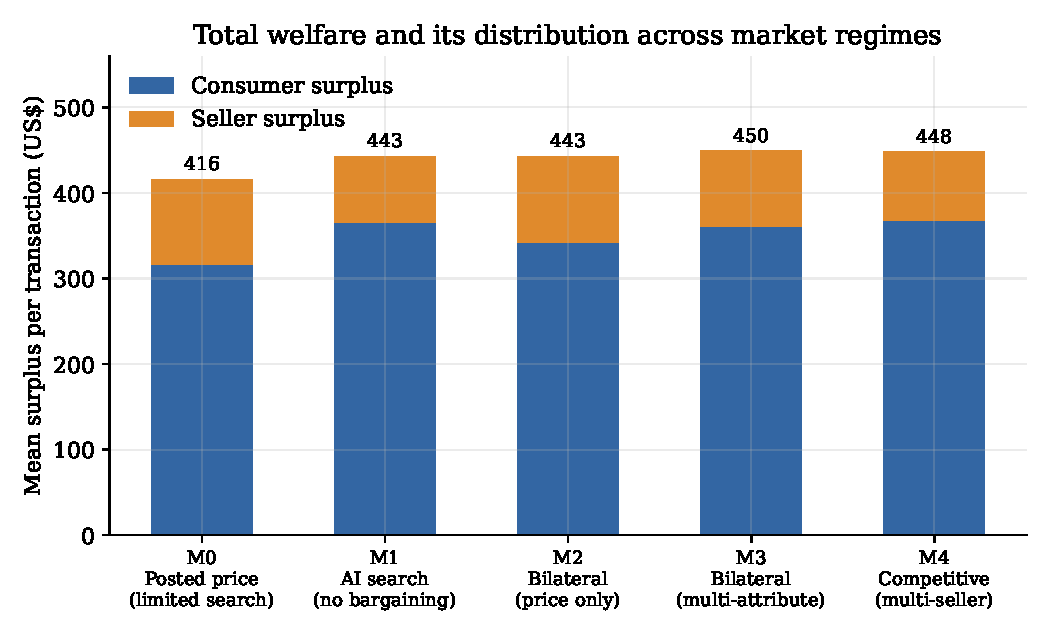
\includegraphics[width=0.85\linewidth]{../figures/fig1_welfare_by_regime.pdf}
\caption{Stacked consumer and producer surplus by institutional regime.}
\label{fig:fig1}
\end{figure}

\begin{figure}[htbp]
\centering
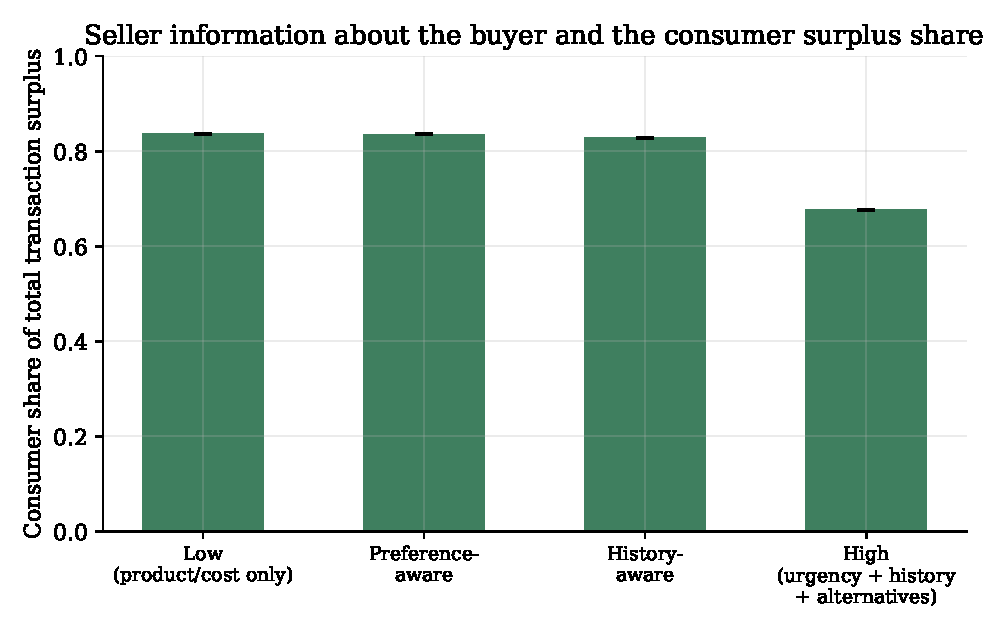
\includegraphics[width=0.85\linewidth]{../figures/fig2_information_csshare.pdf}
\caption{Consumer surplus share as a function of seller information about the buyer.}
\label{fig:fig2}
\end{figure}

\begin{figure}[htbp]
\centering
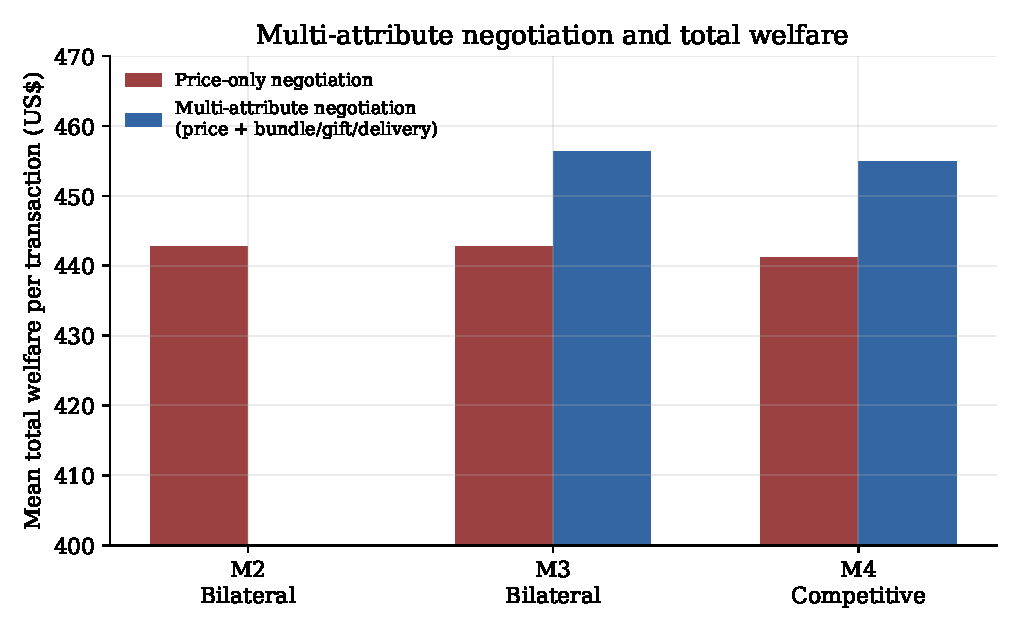
\includegraphics[width=0.85\linewidth]{../figures/fig3_multiattribute_welfare.pdf}
\caption{Welfare under price-only versus multi-attribute bargaining scope, by regime.}
\label{fig:fig3}
\end{figure}

\begin{figure}[htbp]
\centering
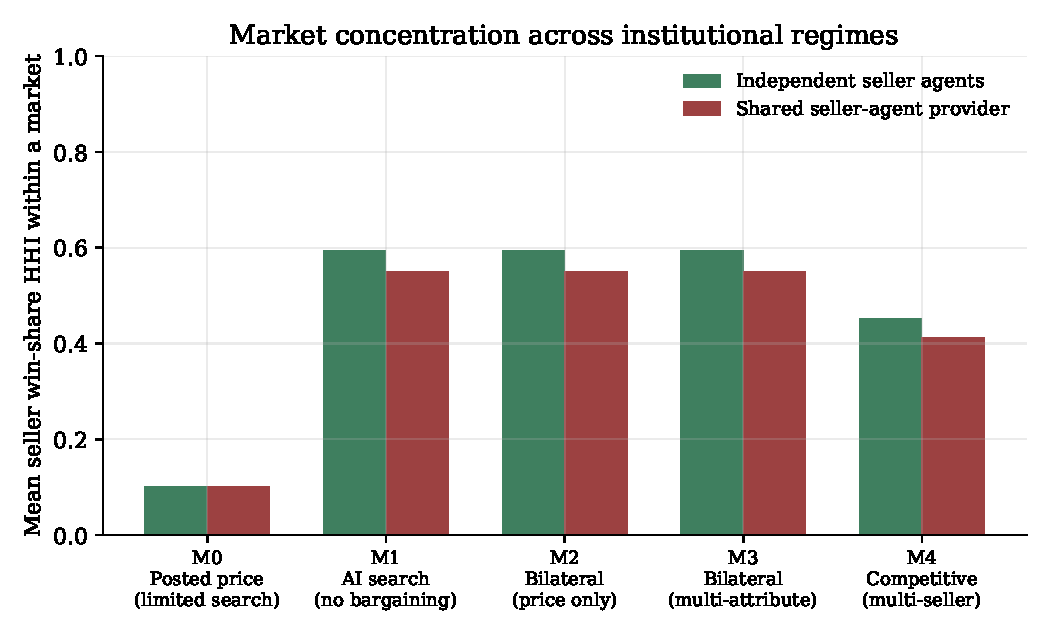
\includegraphics[width=0.85\linewidth]{../figures/fig4_hhi_by_regime.pdf}
\caption{Herfindahl-Hirschman index of seller win-shares by regime and seller-agent concentration.}
\label{fig:fig4}
\end{figure}

\FloatBarrier
\section{Discussion}
\label{sec:discussion}

The results in Section~\ref{sec:results} add up to a more specific claim than "AI agents will change e-commerce," and it is worth stating that claim in the terms \citet{bichler2026agentic} uses to frame the same question: gains from agentic markets are not automatic, and this paper's contribution is to locate precisely where, inside a single consistent environment, they are automatic and where they are not. Search is close to automatically welfare-improving, because giving a buyer's agent access to the whole market rather than a small sample of it is close to a pure information improvement. Bargaining is not automatically welfare-improving on top of that search; it is close to purely redistributive unless the bargaining space is deliberately widened to include attributes beyond price, in which case it becomes a genuine source of new value. That distinction between search, price bargaining, and scope-expanding bargaining is exactly the kind of institutional granularity that the Coasean Singularity argument of \citet{shahidi2025coasean} anticipates in principle, and this paper supplies a quantitative decomposition of it in one concrete setting.

The information result in Section~\ref{sec:results-info} is the paper's clearest illustration of why "agentic commerce" cannot be evaluated as a single undifferentiated technology from a consumer-welfare standpoint. The same AI agent that delivers the search-efficiency gains of Section~\ref{sec:results-search} is, if it is also allowed to infer a buyer's urgency and purchase history, the mechanism by which a seller's agent captures nearly a third of the surplus that a low-information seller would have left with the buyer. A platform, or a regulator, that wants the efficiency gains of agentic search without the extraction risk of agentic personalization cannot get both by simply deciding whether or not to "allow AI agents"; it has to decide, specifically, what information a seller's agent is permitted to infer and act on, a much more granular and more actionable design question than the current policy conversation about AI and e-commerce typically poses.

The concentration results in Sections~\ref{sec:concentration} through~\ref{sec:results-sellerconc} speak directly to the competition-policy literature this paper reviewed in Section~\ref{sec:litreview-collusion}, and to \citet{bostoen2026futureproof}'s question of whether existing regulation anticipates a world of autonomous negotiating agents. Search-driven concentration (Section~\ref{sec:concentration}) is a genuine, sizable effect -- a roughly sixfold increase in the seller win-share Herfindahl index -- but it is a consequence of efficient matching working as intended, not of any anticompetitive conduct, and the simulation shows a concrete, non-regulatory remedy already available to platform designers: requiring or defaulting to competitive multi-seller solicitation (M4) meaningfully reverses much of that concentration without giving up the multi-attribute welfare gains of Section~\ref{sec:results-search}.

The seller-infrastructure result (Section~\ref{sec:results-sellerconc}) requires more interpretive caution than the paper's earlier framing allowed for. It is true, and worth restating plainly, that this paper's simulation contains no repeated-game punishment mechanism, no signaling channel, and no learning dynamic of the kind studied by \citet{calvano2020artificial} or \citet{klein2021autonomous}, so the correlation documented here is not evidence of the specific \emph{tacit-collusion-via-independent-learning} mechanism those papers formalize. But that is a narrower claim than "not collusion" tout court, and the distinction matters for how a competition authority would actually approach this fact pattern. \citet{harrington2026hubandspoke} shows that a third-party pricing algorithm distributing a common pricing policy to multiple, otherwise-competing sellers can sustain hub-and-spoke collusion without any signaling or communication between the sellers themselves -- which is structurally closer to this paper's own mechanism (sellers inheriting correlated strategy parameters from a shared vendor) than to Calvano-style independently-learning agents, and is also the fact pattern underlying recent hub-and-spoke enforcement actions against shared algorithmic pricing vendors in other markets. A real deployed pricing-agent vendor could plausibly combine both mechanisms at once -- a shared trained policy \emph{and} adaptive, repeated interaction among its client sellers' instances -- in which case this paper's clean separation between "correlated parameters" and "learned tacit collusion" is a property of choosing to model only one mechanism at a time, not evidence that the two do not co-occur in practice. The right regulatory takeaway is therefore not that shared seller-agent infrastructure is exonerated by the absence of a repeated-game mechanism in this particular model, but that regulators should look for the specific mechanism at work in a given vendor relationship -- distributed common parameters, adaptive repeated interaction, or both -- rather than treating price correlation as either automatically damning or automatically benign.

Whether the current EU Digital Markets Act is well positioned to do that is a fair question to ask of this paper's findings, and \citet{bostoen2026futureproof} raise it directly, but this paper's own evidence bears on it only indirectly: nothing in the simulation speaks to gatekeeper-designation thresholds, self-preferencing obligations, or interoperability mandates as such. What the seller-concentration finding does suggest, concretely, is that a shared third-party agent-infrastructure vendor -- as distinct from the marketplace platforms the DMA's gatekeeper criteria are built around -- can be the operative locus of coordinated pricing behavior even when no single marketplace is dominant, which is at minimum a reason to ask whether agent-infrastructure providers, and not only marketplaces, warrant scrutiny under a similar framework.

The buyer-side monopsony result (Section~\ref{sec:results-buyerconc}) is smaller in magnitude than any of the above but is arguably the most forward-looking, since it is the one result in this paper that scales with adoption in a way the others do not automatically: if a small number of buyer-agent platforms eventually intermediate a large share of retail transactions, the aggregated bargaining leverage documented here at a 70-percent penetration rate inside one condition could plausibly grow. This is no longer only a speculation: Section~\ref{sec:robustness} reports a direct sweep of buyer-agent-provider penetration from 30\% to 90\%, and the market-average consumer surplus share does rise monotonically over that range, from 0.768 to 0.771 -- a modest but consistently signed effect, converting what was previously an untested extrapolation into an actual, if still small, data point, and one consistent with the countervailing-power mechanism documented empirically in other bilateral-bargaining settings by \citet{chipty1999role}.

Two stakeholder groups are notably absent from the welfare accounting above, and both are worth naming rather than leaving implicit. First, this paper's sellers are modeled as symmetric utility-maximizing principals, but in practice the sellers most likely to end up on a low-tier, heavily shared third-party pricing-agent provider are small merchants who cannot afford bespoke agent infrastructure -- for them, the "shared-infrastructure" condition this paper treats as a pricing-correlation curiosity (Section~\ref{sec:results-sellerconc}) is also an access-inequality story about which sellers get a sophisticated negotiating agent at all. Second, this paper's buyers are modeled as either on a common provider or fully independent, but never as lacking a capable agent altogether; the consumer-surplus gains documented throughout Section~\ref{sec:results} accrue specifically to buyers equipped with an AI shopping agent, and nothing in the model speaks to consumers who cannot afford, trust, or operate one -- a digital-divide dimension that this paper's aggregate welfare numbers do not, and by construction cannot, capture.

\section{Limitations}
\label{sec:limitations}

The central limitation of this paper is one it has tried to state honestly throughout rather than discover in a closing section: the primary empirical engine is a rule-based agent-based computational economics simulation, calibrated qualitatively to the mechanisms described in the agentic-commerce literature but not fit to, or validated against, any specific deployed large language model or commercial AI shopping agent. The supplementary LLM-agent pilot in Sections~\ref{sec:methodology-llm} and~\ref{sec:results-llm} provides a small, genuinely encouraging piece of corroborating evidence that the paper's central bundling result is not an artifact of the rule-based model's particular functional form, but thirty-six episodes across three model pairings is an exploratory check, not a validation study, and Section~\ref{sec:results-llm} discusses directly why the pilot's own inconvenient unconditional result cannot be fully ruled out as evidence that multi-attribute negotiation is genuinely, not just incidentally, harder for real language models to close.

Several further limitations follow from the simulation's design choices. Buyer valuations, seller costs, and bundle values are drawn from stylized, independent uniform distributions calibrated for tractability and interpretability rather than fit to any real product category's actual price and cost data. Rather than simply asserting that the qualitative ordering of results (search improves matching, price-only bargaining redistributes, multi-attribute bargaining creates surplus) is robust to reasonable changes in these distributions, Section~\ref{sec:robustness} tests this directly for the parameter identified as most consequential -- the ratio of a bundle's provision cost to its value -- and finds that H3's direction holds across a wide range of that ratio but is not unconditional: it weakens as bundles become more expensive to provide and reverses sign once bundle cost approaches bundle value. The paper has not similarly re-run the full factorial design under alternative shapes for the underlying cost and valuation distributions (e.g., log-normal in place of uniform), which remains an open robustness question; the specific magnitudes reported throughout -- the 13.6-unit welfare gain, the fall from 84 to 68 percent in consumer surplus share -- are properties of the paper's particular calibration and should not be read as forecasts for any specific real market even where the qualitative direction is well supported. The simulation also studies a single, homogeneous product category; real e-commerce spans categories with very different search costs, negotiation norms, and repeat-purchase dynamics, and nothing in this paper's design speaks to how these results would generalize across categories. Finally, the paper works entirely with simulated rather than real transaction data, a consequence of the fact that autonomous buyer-seller agent negotiation, in the full sense studied here, is not yet observable at the scale or with the institutional variation this paper's design requires; validating these mechanism-level predictions against real transaction data, as agentic commerce platforms mature and such data becomes available, is the natural and necessary next step this paper's own approach cannot take on its own.

\section{Conclusion}
\label{sec:conclusion}

This paper set out to ask whether the arrival of AI shopping and pricing agents matters for e-commerce markets because of what those agents are, or because of the specific institutional rules under which they are allowed to search, bargain, and share information. The evidence assembled here, from a matched, fully reproducible simulation of 105,600 transactions and a smaller corroborating pilot with real language models, comes down clearly on the side of institutional rules. Search is close to automatically beneficial; price-only bargaining is close to purely redistributive; multi-attribute bargaining is where genuine efficiency gains are created; seller information is where those gains are put at risk of being extracted from the buyer who helped create them; and agent-provider concentration, on both sides of the market, leaves real but importantly different fingerprints depending on whether it is the buyer's side or the seller's side that is concentrated. None of these findings depends on any single AI system's particular training or prompting; all of them depend on design choices -- how many sellers a shopping agent solicits, what a pricing agent is allowed to infer, how wide the negotiation space is allowed to be -- that platform designers and regulators are making, or will soon be making, right now. The paper's central practical claim is that those design choices, not the underlying presence of AI, are where the welfare and competition consequences of agentic commerce will actually be decided.

\section*{CRediT authorship contribution statement}
The author is solely responsible for all aspects of this work: conceptualization, methodology, software, validation, formal analysis, investigation, data curation, writing of the original draft, writing review and editing, and visualization.

\section*{Declaration of competing interest}
The author declares no known competing financial interests or personal relationships that could have appeared to influence the work reported in this paper.

\section*{Funding}
This research received no specific grant from any funding agency in the public, commercial, or not-for-profit sectors.

\section*{Data availability}
The simulated transaction dataset, the LLM-agent negotiation pilot's episode data and transcripts, and all simulation, analysis, and figure-generation code that support the findings of this study are openly available in a public code repository. A repository link will be provided upon acceptance to preserve the integrity of the double-anonymized review process.

\section*{Declaration of Generative AI and AI-assisted technologies in the writing process}
During the preparation of this work, the author used Claude (Anthropic) to assist with the design and implementation of the agent-based simulation code, the statistical analysis and figure-generation scripts, the implementation of the supplementary LLM-agent negotiation pilot, and the drafting and editing of portions of this manuscript's text. The author reviewed, verified, and edited all AI-assisted content, independently confirmed all reported numerical results against the underlying code and data outputs, and takes full responsibility for the content of this publication.

\bibliography{references}

\end{document}
